\logvartrue
\chapter{Other applications of the computational tools}
\label{sec:appendix1}

\section{Enly: improving draft genomes through reads recycling}
The reconstruction of the complete genome sequence of an organism is a key point for comparative, functional and evolutionary genomics. Nevertheless, overcoming the problems encountered while completing the sequence of an entire genome is still highly demanding in terms of time and resources.
We have developed a tool (named Enly) based on the iterative mapping of sequence reads at contig edges, capable to extend the genomic contigs deriving from high-throughput 454 sequencing and Newbler assembler. We tested Enly performances in improving the assemblies of bacterial genomes sequenced by 454 pyrosequencing platform and it allowed the automated closure of about 10\% of the gaps for each of the bacterial draft genomes.
In this work we present Enly, a software allowing the extension of draft genomes contigs resulting from de novo assembly and thus being helpful during genomes finishing procedures. Enly is particularly suited to be used with long (length > 200nt) reads and with assemblers that trim contigs ends. Enly and its related documentation can be downloaded at \href{http://enly.sf.net}{http://enly.sf.net}\footnote{Marco Fondi, Valerio Orlandini, Giorgio Corti, Marco Severgnini, \textbf{Marco Galardini}, Alessandro Pietrelli, Fabio Fuligni, Michele Iacono, Ermanno Rizzi, Gianluca De Bellis and Renato Fani}.

\subsection{Introduction}
The advent of the so-called next-generation-sequencing (NGS) platforms has allowed the scientific community to approach the genome sequencing of a huge number of organisms, species and strains at reasonable costs. Indeed, determining the entire genome sequence of an organism is one of the key steps in elucidating the details of its biology, and it is also propaedeutic for a plethora of additional analyses (such as structural genomics, transcriptomics, SNPs detection) that require a complete genome sequence or, at least, a good quality draft assembly. Hence, sequence assembly is the first challenge encountered in a typical computational genomics pipeline and involves the merging and the ordering of shorter sequence fragments (reads) with the aim to get as close as possible to the original larger sequence (genome). However, many issues regarding the computational assembly of large-scale sequencing data have remained unsolved \cite{scheibye2009sequence} and, actually, the number of draft genomes in databases greatly overtakes the number of completely sequenced (closed) ones (\href{www.genomesonline.org}{www.genomesonline.org}). The output of a de novo assembly is typically a draft genome, consisting of a set of contigs (i.e. contiguous sequence fragments) that may be ordered and oriented into scaffold sequences, with gaps between them, representing regions of uncertainty \cite{earl2011assemblathon}. This may be due to several causes, including the presence of repetitive fragments along the genome and/or the absence of enough reads to produce a reliable assembly, according to the de novo assembler parameters. Approaching gaps closure in genomes (even bacterial ones) is a time-consuming and not easily automated effort, often involving the setup and the execution of a series of PCR reactions \cite{galardini2011contiguator}. Thus, pushing towards the limits of the in-silico sequence reconstruction is desirable in order to reduce the amount of laboratory work to be done after the completion of the bioinformatic procedures. Some traditional assemblers like Newbler (454 Sequencing, Roche Diagnostics, Indianapolis, IN, USA) usually perform a trimming of the contig edges depending on the quality of the supporting reads. This conservative procedure, however, may result in a loss of information, discarding many correct bases characterized by a sub-optimal quality. To overcome these limitations, we have developed a tool called Enly that allows increasing the length of the contigs deriving from Newbler assemblies and the closure of some of the gaps commonly present in the draft genome.

\subsection{Results and discussion}
\begin{figure}[!tb]
	\center
    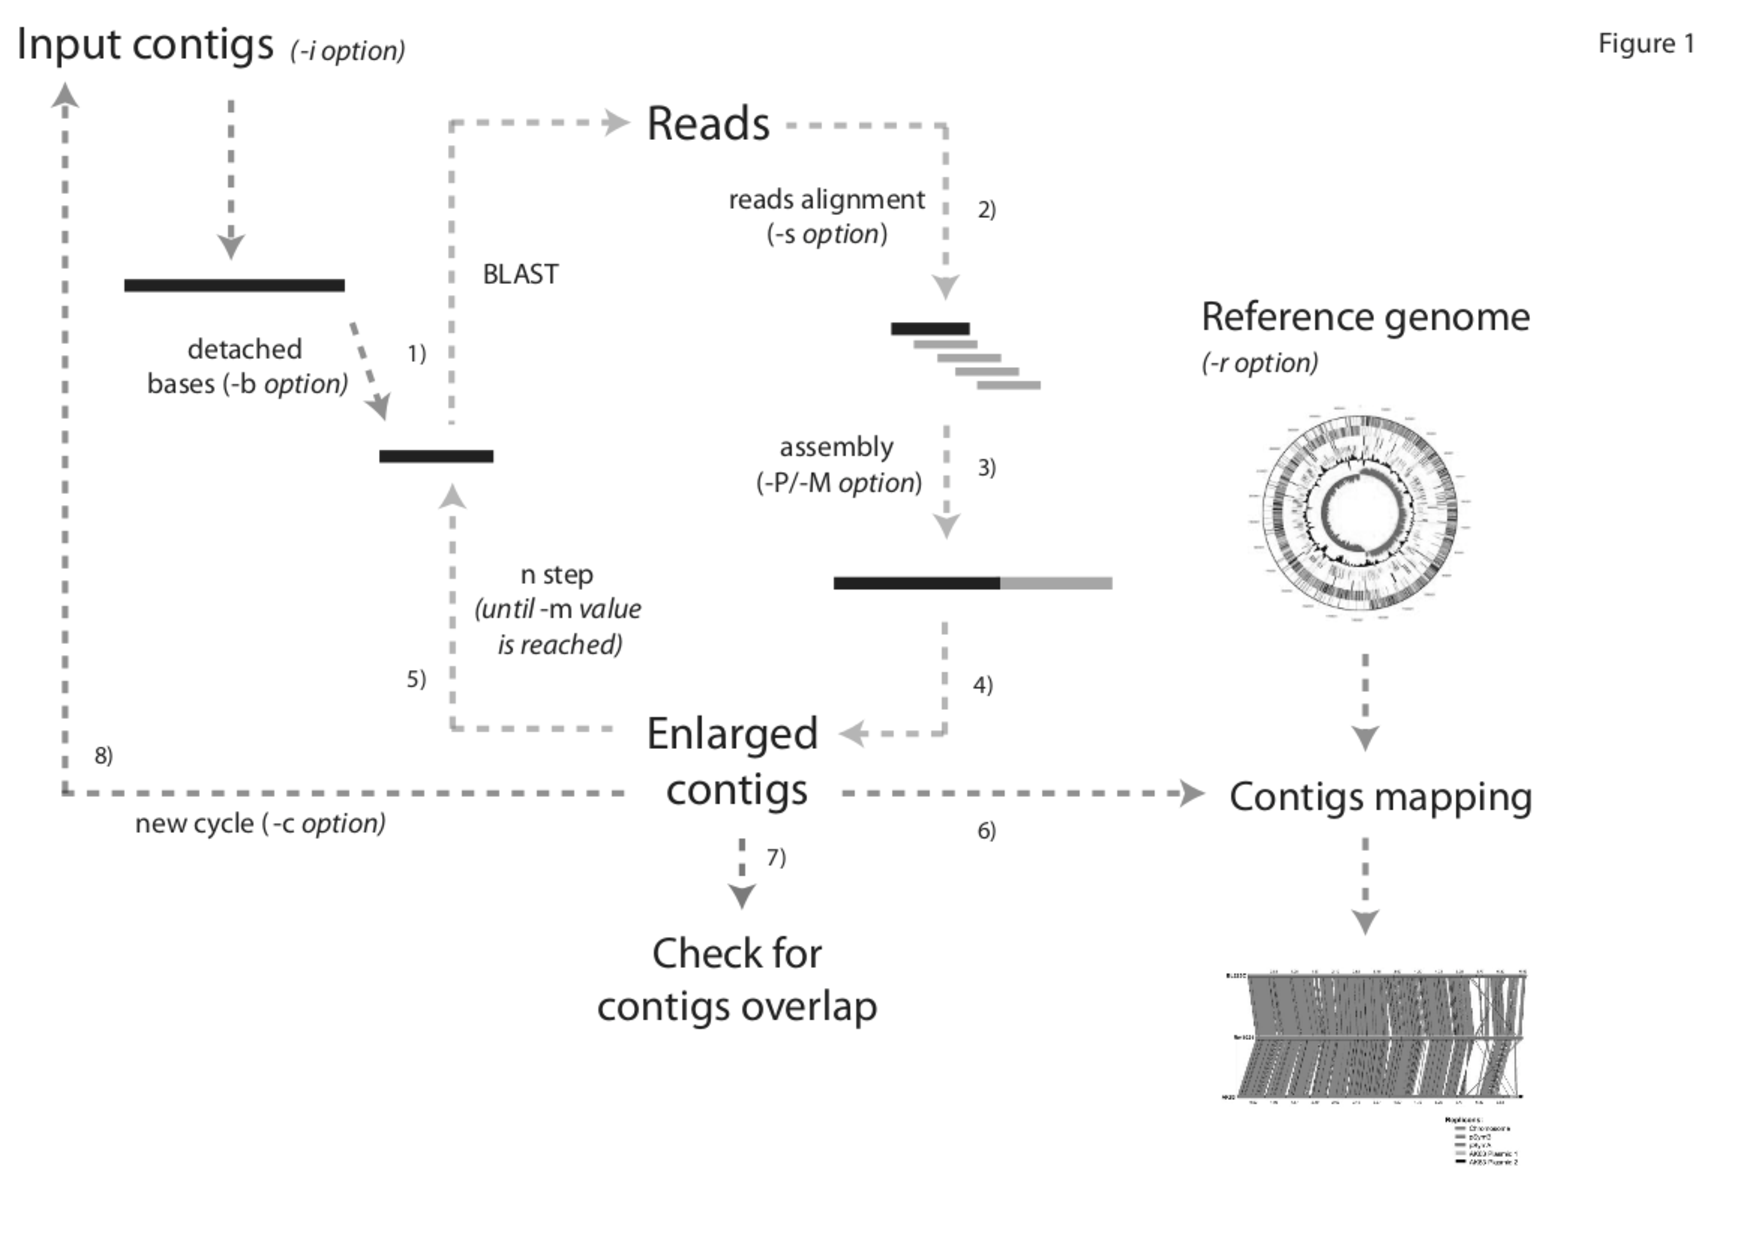
\includegraphics[width=1\textwidth]{figures/appendix/thesis_36}
	\caption{\label{fig:enly}\textbf{A schematic representation of the whole Enly pipeline together with the specific role of each parameter}}
\end{figure}

Enly is based on the iterative mapping of reads at the edges of contigs obtained after de novo assembly using Newbler or similar tools, characterized by the qualitative trimming of the contig extremities during the assembly. Enly is made up of a central core (named autoenlarge) written in C++ and by other Perl and Python modules that complete the whole pipeline (Figure \ref{fig:enly}). The computational time required for contigs extension and mapping obviously correlates with the number of contigs/reads in the input files and the number of cycles/steps (see below) specified by the user. The computational time on a machine with eight 3.1 GHz processors for the tests performed in this work (see below) ranged from 2 hours for the smallest dataset to 5 hours for the largest.
The overall procedure requires (at least) two multi-fasta files as input, one containing all the contigs deriving from the first assembly and the other all the raw reads resulting from the sequencing run. By applying the strategy described below to each contig in the input file, Enly tries to increase their length and (possibly) to merge them into scaffolds.
More in detail, the pipeline is based on the iteration of multiple cycles (Figure \ref{fig:enly}) and during each of them:
\begin{enumerate}
\item A fragment of length l1 (specified by the user) is detached from the 5’-end of each contig and is used as an input for a BLAST search \cite{camacho2009blast+} against a database embedding all the raw reads resulting from the sequencing run;
\item The BLAST output is parsed to identify reads that can be used to extend the contig (i.e. those partially aligned at the end of the contig and protruding from its extremity);
\item The identified reads and the original contig are assembled together using either Phrap \cite{machado2011phred} or Minimo \cite{treangen2011next} assemblers, possibly resulting in an “enlarged” contig (i.e. contig of increased length);
\item The very same procedure is repeated for the 3’-end of the contig and for all the other contigs of the input file;
\item The extended contigs are used as inputs for a second step, in which a fragment of length l2 (with l2< l1) is detached from each contig end and used as an input for a further BLAST against the reads database, assembling the matching reads with the enlarged contig. This procedure, performed in order to compensate for the presence of reads with a heterogeneous length distribution (resulting from a typical 454 run \cite{margulies2005genome}), is repeated for fragments of decreasing length, until the minimum length (specified by the user) has been reached;
\item If a reference genome (in fasta format) has been provided by the user, the contigs are mapped onto it, taking advantage of an ad hoc modified version of the CONTIGuator tool \cite{galardini2011contiguator};
\item When all the contigs have been processed through these steps, they are mapped one against each other for determining the eventual overlap and the closure of previously present gaps.
\end{enumerate}
The first cycle of the Enly pipeline is completed when all the contigs have been processed, mapped and saved to a new multi-fasta file. The procedure is then repeated (re-starting from point 1) for a user-specified number of cycles or, alternatively, until no more bases have been added to the contigs during the last cycle. Output files from the mapping procedure are saved in separate folders (one per cycle), ready for being loaded by the Artemis Comparison Tool \cite{carver2005act} in order to check the presence of eventual mis-assemblies.

To evaluate the reliability of the pipeline, we tested Enly on three different 454 reads datasets retrieved from either the NCBI short read archive database (SRA, \href{http://www.ncbi.nlm.nih.gov/sra}{http://www.ncbi.nlm.nih.gov/sra}), namely \textit{Escherichia coli} KO11 (SRS084754), \textit{Staphylococcus aureus} 649 (SRS114535) or from a previous sequencing run on \textit{Streptococcus pneumoniae} AP200 \cite{romina11complete}. For these reads datasets the corresponding complete genomes (E. coli KO11 and \textit{S. pneumoniae} AP200 \cite{romina11complete}\cite{turner2012optical}) or the genome of a phylogenetically close bacterium (\textit{S. aureus} COL \cite{gill2005insights}) were available, allowing the validation of the results obtained with Enly. Each reads dataset was first assembled with Newbler v. 2.6, using default parameters, resulting in 719, 254 and 124 contigs for \textit{E. coli} KO11, \textit{S. aureus} 649 and \textit{S. pneumoniae} AP200, respectively. Contigs obtained from de novo assembly were then used, together with the corresponding reads, as input for the Enly pipeline.

\begin{sidewaystable}[htbp]
  \centering
    \begin{tabular}{rrrrrrr}
    \toprule
    Strain name & Genome size (Mb) & N.  reads & Av. reads length & N.contigs & Added bases & Closed gaps \\
    \midrule
    \multicolumn{1}{c}{KO11} & \multicolumn{1}{c}{4.92} & \multicolumn{1}{c}{339,22} & \multicolumn{1}{c}{215.7} & \multicolumn{1}{c}{719} & \multicolumn{1}{c}{51,288} & \multicolumn{1}{c}{54(7.5 \%)} \\
    \multicolumn{1}{c}{649} & \multicolumn{1}{c}{2.80} & \multicolumn{1}{c}{122,569} & \multicolumn{1}{c}{245.6} & \multicolumn{1}{c}{254} & \multicolumn{1}{c}{32,446} & \multicolumn{1}{c}{27(10.6\%)} \\
    \multicolumn{1}{c}{AP200} & \multicolumn{1}{c}{2.13*} & \multicolumn{1}{c}{152,452} & \multicolumn{1}{c}{231.2} & \multicolumn{1}{c}{124} & \multicolumn{1}{c}{29,798} & \multicolumn{1}{c}{12(9.6\%)} \\
    \bottomrule
    \end{tabular}%
  \caption{\textbf{Enly results on three different reads dataset}\\
  		Enly performances after one cycle on three different 454 reads datasets, \textit{E. coli} KO11, \textit{S. aureus} 649 and \textit{S. pneumoniae} AP200. Percentages in parentheses indicate the relative number of closed gaps in respect to the ones originally present in the draft genome}
  \label{tab:enly}%
\end{sidewaystable}%

In all cases, Enly was able to improve the de novo assembly (Table \ref{tab:enly}). In particular, 12, 27 and 54 gaps were closed after one cycle of Enly, on \textit{S. pneumoniae} AP200, \textit{S. aureus} 649 and \textit{E. coli} KO11 contigs, respectively, and representing about 10\% of the gaps originally present in the draft genomes. Notably, a large amount of sequence was added to the de novo assemblies, ranging from more than 50000 bases in the cases of \textit{E. coli} KO11 to roughly 30000 in the cases of \textit{S.aureus} 649 and \textit{S. pneumoniae} AP200 genomes. In order to validate Enly results (i.e. the correctness of the overlaps identified among the extended contigs), we mapped the originally assembled contigs (i.e. before using them as input for Enly) on the corresponding complete genome sequence using Mauve \cite{darling2004mauve} with default parameters. These mapping results were compared to the positioning of the Enly-derived contigs, confirming the correctness of both the extensions and the gap closures. Iterating the algorithm of Enly for more than 1 cycle, allowed assembling even more sequence to the contigs (14517, 8411 and 37966 bases to \textit{S. pneumoniae} AP200, \textit{S. aureus} 649 and \textit{E. coli} KO11, respectively), although it did not lead to the closure of novel gaps in respect to the first cycle. 
Finally, to determine the influence of reads average length on the overall performances of the pipeline, we performed a further test on a 454 reads dataset from the 3.6 Mb genome of A\textit{cinetobacter baylyi} ADP1 (SRA id: SRX001813) whose reads were characterized by an average read length of 184 bp (thus sensibly shorter in respect to the other datasets). When tested on this dataset, Enly added 72,498 bp to the draft genome, although allowing the closure of only 2 gaps (data not shown).

Commonly-used genome finishing tools typically allow the mapping of de novo contigs on a reference genome (e.g., Projector 2 \cite{van2005projector}, CONTIGuator \cite{galardini2011contiguator}, Mauve \cite{darling2004mauve}) but very few allow to extend contigs using the original reads before mapping them. Recently, two scaffolding approaches, apparently similar to the one presented here, which take advantage of the additional information that is present on a typical Illumina paired-end sequencing run \cite{boetzer2012toward}\cite{tsai2010improving} have been developed. Nevertheless, Enly does not require a paired-end sequencing, being specifically designed for single end sequencing runs. Moreover, the pipeline does not rely on the presence of a reference genome to perform contig extension. However, since the availability of a complete genome from a closely related organism may facilitate genome closure and the identification of mis-assemblies, an optional tool (based on the CONTIGuator pipeline) to map contigs on a reference genome (if any) has been added to the overall pipeline.

\subsection{Conclusions}
Enly is a simple, cross-platform and parallelizable tool allowing the improvement of draft genomes resulting from Newbler-assembled 454 high-throughput sequencing reads. It has been shown to be particularly suited for long reads (greater than 200 bp) allowing the automated closure of about 10\% of the gaps within bacterial draft genomes, thus resulting helpful during genomes finishing procedures. The software has been developed and tested to improve genome assemblies resulting from high-throughput 454 sequencing and Newbler assembler, although, in principle, it allows the use of a large variety of read types for contig extension, including those resulting from classical sequencing methods (e.g. Sanger) or hybrid datasets, embedding a mixture of reads obtained with different technologies.

\newpage
\section{The clinical success of \textit{Acinetobacter} species: genetic, metabolic and virulence attributes}
The flexibility of the analysis methods that have been implemented in the DuctApe software suite (see section \ref{sec:ductape}) is demonstrated with the comparative genomics and phenomics study on the pathogenic \textit{Acinetobacter} species: the genomic data from four \textit{Acinetobacter} strains have been combined with the complete analysis on their phenotypes, using the Phenotype Microarray plates, in order to obtain a general view on the main metabolic differences and also to give some insights on the genetic determinants of these differences.

\newpage
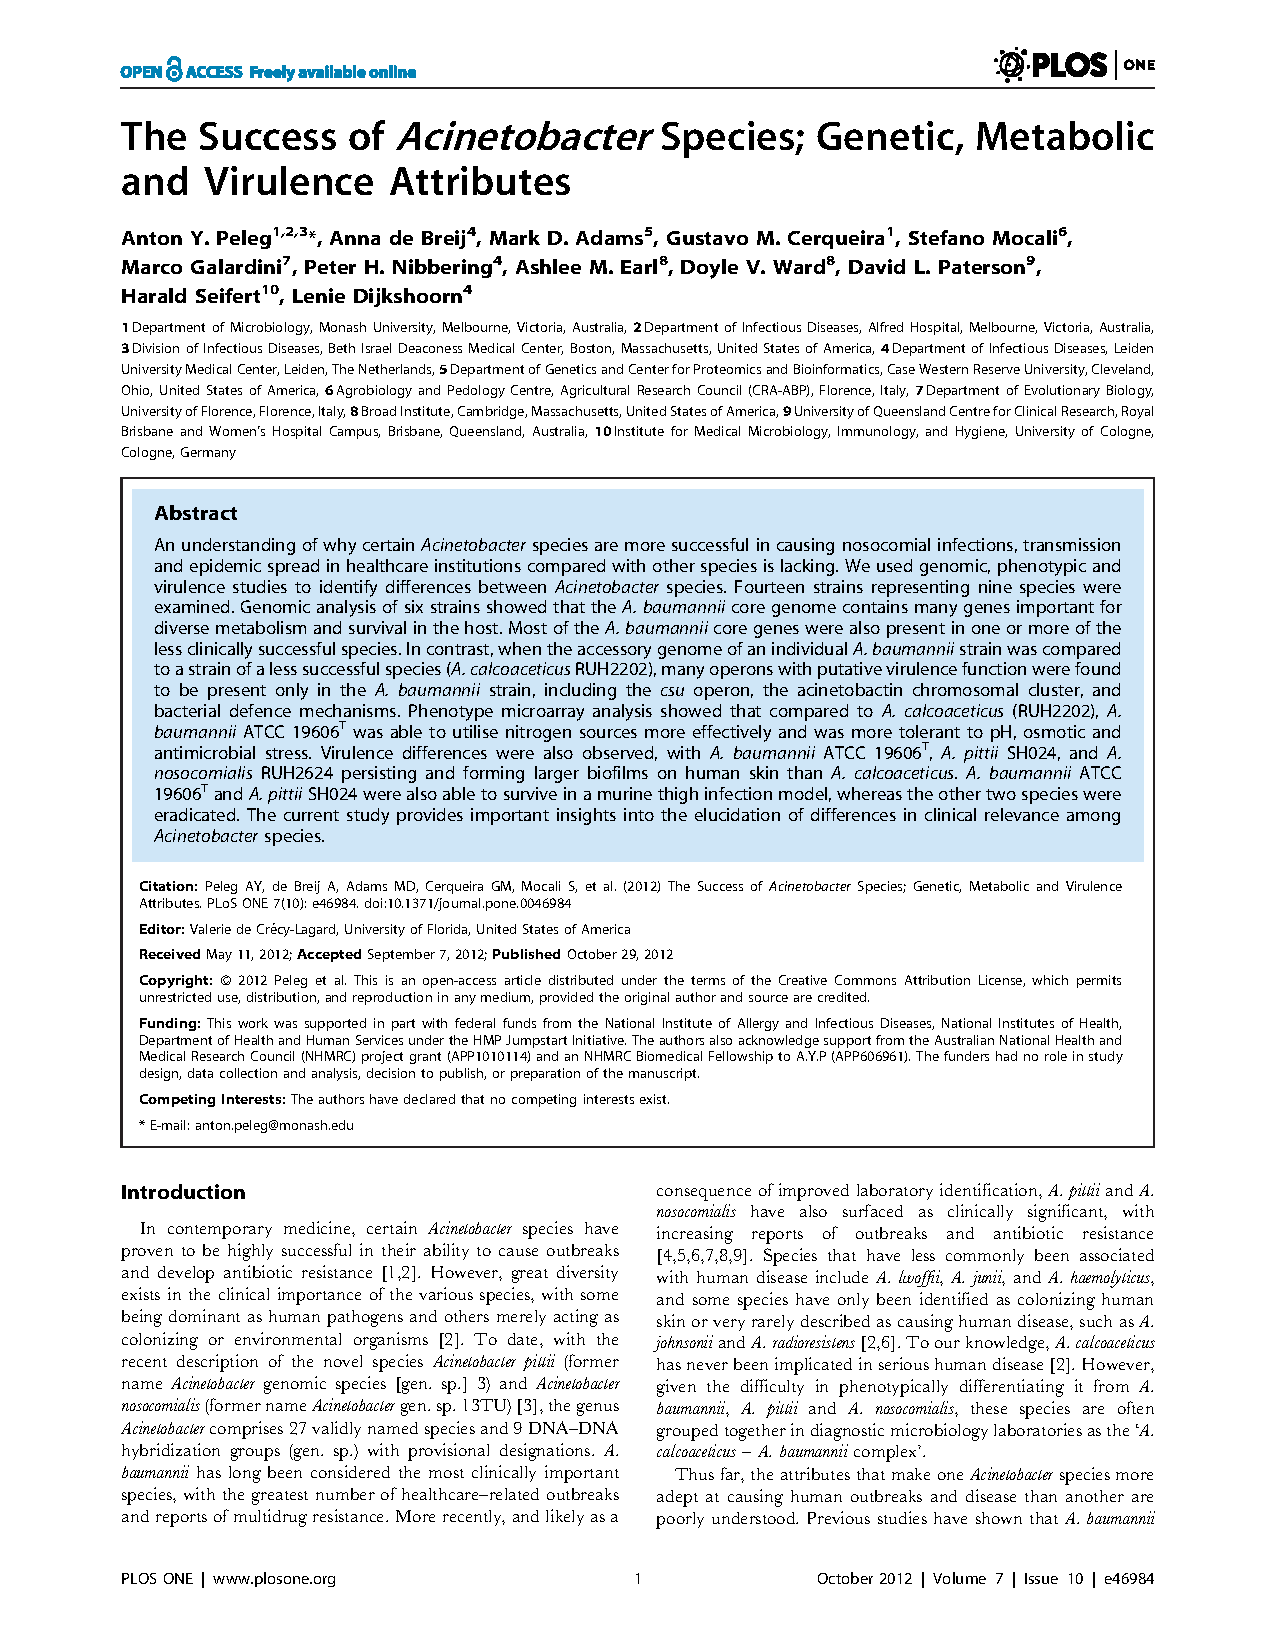
\includepdf[pages=-,offset=10mm 0, scale=0.9]{articles/Peleg2012.pdf}


%%-----------
%% Backmatter
%%-----------
\backmatter
\chaptermark{Bibliography}
\renewcommand{\sectionmark}[1]{\markright{#1}}
\bibliographystyle{unsrt}                           %Use alpha codes for references
\sectionmark{Bibliography}
\addcontentsline{toc}{chapter}{Bibliography}        %Force addition of Bibliography to TOC    
\bibliography{References}